%!BIB TS-program = biber
\documentclass[11pt]{article}%
\usepackage{amsmath}
\usepackage{amsfonts}
\usepackage{amssymb,tcolorbox}
\usepackage{graphicx}
\usepackage{amssymb}%
\usepackage{siunitx}
\usepackage{listings}
\usepackage[style=ieee]{biblatex}
\setcounter{MaxMatrixCols}{30}
\providecommand{\U}[1]{\protect\rule{.1in}{.1in}}
\providecommand{\U}[1]{\protect\rule{.1in}{.1in}}
\providecommand{\U}[1]{\protect\rule{.1in}{.1in}}
\newtheorem{theorem}{Theorem}
\newtheorem{acknowledgement}[theorem]{Acknowledgement}
\newtheorem{algorithm}[theorem]{Algorithm}
\newtheorem{axiom}[theorem]{Axiom}
\newtheorem{case}[theorem]{Case}
\newtheorem{claim}[theorem]{Claim}
\newtheorem{conclusion}[theorem]{Conclusion}
\newtheorem{condition}[theorem]{Condition}
\newtheorem{conjecture}[theorem]{Conjecture}
\newtheorem{corollary}[theorem]{Corollary}
\newtheorem{criterion}[theorem]{Criterion}
\newtheorem{definition}[theorem]{Definition}
\newtheorem{example}[theorem]{Example}
\newtheorem{exercise}[theorem]{Exercise}
\newtheorem{lemma}[theorem]{Lemma}
\newtheorem{notation}[theorem]{Notation}
\newtheorem{problem}[theorem]{Problem}
\newtheorem{proposition}[theorem]{Proposition}
\newtheorem{remark}[theorem]{Remark}
\newtheorem{solution}[theorem]{Solution}
\newtheorem{summary}[theorem]{Summary}
\newenvironment{proof}[1][Proof]{\noindent\textbf{#1.} }{\ \rule{0.5em}{0.5em}}
\addtolength{\oddsidemargin}{-.875in}
\addtolength{\evensidemargin}{-.875in}
\addtolength{\textwidth}{1.75in}
\addtolength{\topmargin}{-1in}
\addtolength{\textheight}{2in}
\usepackage{tocloft}
\usepackage{color} %red, green, blue, yellow, cyan, magenta, black, white
\definecolor{mygreen}{RGB}{28,172,0} % color values Red, Green, Blue
\definecolor{mylilas}{RGB}{170,55,241}

\addbibresource{proj4.bib}

\title{MANE 6710 - Numerical Design Optimization Lab 4}
\author{Human 6966}
\date{December 10 2024}

\renewcommand{\contentsname}{Table of Contents:}
\setcounter{tocdepth}{2} % Include sections and subsections
\setlength{\cftbeforesecskip}{0.5cm} % Adjust spacing between entries
\begin{document}
\maketitle
\newpage
\tableofcontents
\newpage
\addcontentsline{toc}{section}{Executive Summery}
\section*{Executive Summery}
\label{sec:abstract}

Wing spars are an important part of aviation design because they support the loading of airplane wings, enabling airplanes to stay in the air. These must be as light as possible as this increases the load capacity of the aircraft, which is an important consideration for most aircraft designs. This lab focuses on choosing and using optimization algorithms in Matlab (\lstinline{fmincon()}) along with the complex stem method of approximating gradients to optimize the profile of a wing spar to minimize their mass. A two-dimensional discretized version of the Euler-Bernoulli Beam Theory was chosen to analyze the structural system, and the SQP algorithm for \lstinline{fmincon()} was selected to optimize the profile of the wing spar. To handle uncertainty in the loading of the wing, the first four harmonic modes were added to the loading condition and the design space was limited to designs at least six standard deviations stronger than the mean loading. The SQP algorithm was successfully able to minimize the mass of the wing spar within the problem constraints by minimizing the thickness and outer radius of the spar.

\section{Analysis Introduction}
\label{sec:intro}

\subsection {Methodology}
\label{sec:analysismethod}

The method used to analyze the stress in the beam was the Euler-Bernoulli Beam Bending Theory (see lab two for more information \cite{lab2}). The first four modes of loading perturbation are given by equation \ref{eqn:loadingModes}.

\begin{equation}
\label{eqn:loadingModes}
\delta_{f}(x,\zeta_{n})=\zeta_{n}\cos(\frac{(2n-1)\pi x}{2L})
\end{equation}
with
\begin{itemize}
	\item $\zeta_{n}$ being a normally distributed random variable $N(0,\frac{f_{nom(0)}}{10n})$
	\item n being the mode number (1, 2, 3, or 4)
	\item x being the position along the spar
	\item L being the length of the spar
	\item $f_{nom}(0)$ being the nominal loading at the base of the wind spar
\end{itemize}
These perturbation modes were added to the loading condition used in lab two when calculating the stresses at each point. Then the mean and standard deviation of the stresses were calculated at each node with Gauss-quadrature using equations \ref{eqn:mean} and \ref{eqn:stddev}
\begin{equation}
\label{eqn:mean}
\mu_{i}=\sum_{i1=1}^{m}\sum_{i2=1}^{m}\sum_{i3=1}^{m}\sum_{i4=1}^{m} w_{i1}w_{i2}w_{i3}w_{i4} \eta(q(x_{i1},x_{i2},x_{i3},x_{i4}),R)_{i}
\end{equation}
\begin{equation}
\label{eqn:stddev}
\sigma_{i}=\sqrt{\eta^{2}_{i}-\mu^{2}_{i}}
\end{equation}
with
\begin{itemize}
	\item $\eta_{i}$ being the stress function at node i
	\item $\mu_{i}$ being the mean stress at node i
	\item $w_{iy}$ being the adjusted Gauss quadrature weight for the yth perturbation mode 
	\item $w_{iy}= \frac{w_{x}}{\sqrt{\pi}}$
	\item $w_{x}$ being the standard Gauss quadrature weight \cite{gauss}
	\item $x_{iy}$ being the adjusted Gauss quadrature point for the yth perturbation mode
	\item $x_{iy}= \sqrt{2}x_{z}\frac{f_{nom}(0)}{10n}$
	\item $x_{z}$ being the standard Gauss quadrature point \cite{gauss}
	\item $\sigma_{i}$ being the standard deviation of the stress at node i
\end{itemize}

\subsection{Assumptions}
\label{sec:assumption}
To simplify the physical model and fundamental equations, the following assumptions were made in addition to the ones in lab two \cite{lab2}:
\begin{enumerate}
    	\item The loading perturbation can be represented as a set of harmonic modes
   	 \item The perturbation modes are independent random variables
    	\item The perturbation modes are normal random variables
\end{enumerate}

\subsection{Limitations}

These assumptions limit this analysis method to cases where the loading perturbations can be represented as a Fourier series or integral (which has limited effect as many aerodynamic phenomena can be represented this way). Additionally, it may be experimentally determined that in some cases the harmonic loading perturbation modes aren't normally distributed. For these cases, a new mean and standard deviation model would have to be made as these are only valid for normally distributed random variables. Finally if the perturbation modes are proven to not be independent, a new model for the mean and standard deviation would be required to account for the interaction between random variables.

\section{Parameterization of the Geometry}
\label{sec:parameterization}

The geometry was parameterized  the same way as in lab two \cite{lab2}. A finite element mesh of N+1 nodes was used to represent the geometry with the stress calculated at each node.

\section{Optimization Method and Limitations}
\label{sec:optimizationmethod}

The optimization method from lab two is the same as in this lab except for the nonlinear constraint given by equation \ref{eqn:c}. This means that all of the previous assumptions and limitations hold for this lab (Note that $\eta$ in this lab is equivalent to $\sigma$ in the previous lab).

\begin{equation}
\label{eqn:c}
c(i)=\frac{\mu+6\sigma}{\eta_{ultimate}}-1\leq0
\end{equation}

\section{Optimization Problem}
\label{sec:problem}
The objective of this lab is to apply the principles learned in lecture to optimize the shape of a wing spar modeled within the following criteria and constraints in addition to the ones presented in lab two \cite{lab2}\cite{lab4doc}\cite{lab2doc}:
\begin{enumerate}
	\item $\eta_{ultimate}=600$ MPa
	\item $\mu +6\sigma\leq \eta_{ultimate}$
\end{enumerate}
The objective of this project is to optimize the shape of the wing spar to minimize the weight. The model geometry was parameterized and discretized (see section \ref{sec:parameterization} for more details) and applied to a discretized version of the Euler-Bernoulli Beam Theory to analyze the problem. Gauss quadrature used to calculate the mean and standard deviation of the stress for the nonlinear constraint. The method chosen for the minimization problem was the SQP algorithm for the fmincon Matlab function (see lab two section \ref{sec:optimizationmethod} for more details \cite{matlab}) with the gradients calculated using the complex step method.

\section{Results}

%convergence for Gauss quadrature

The convergence plot shown in Figure \ref{fig:conv} was calculated by taking the norm of the error of $\mu+6\sigma$ at each node using 1, 2, 3, 4, 5, and 6 Gauss quadrature points from the result of using six Gauss quadrature points. The plot shows a significant decrease in error between the first and second set of Gauss quadrature points relative to the six-point solution before remaining relatively flat near zero. This behavior makes sense as it shows the function is closely approximated by a third-order polynomial and thus can be approximated well with a higher-order polynomial but not a lower-order one. The acceptable number of Gauss quadrature points was determined to be two as it represented little error while also not resulting in a long run time.
\begin{figure}[h!]
    \centering
    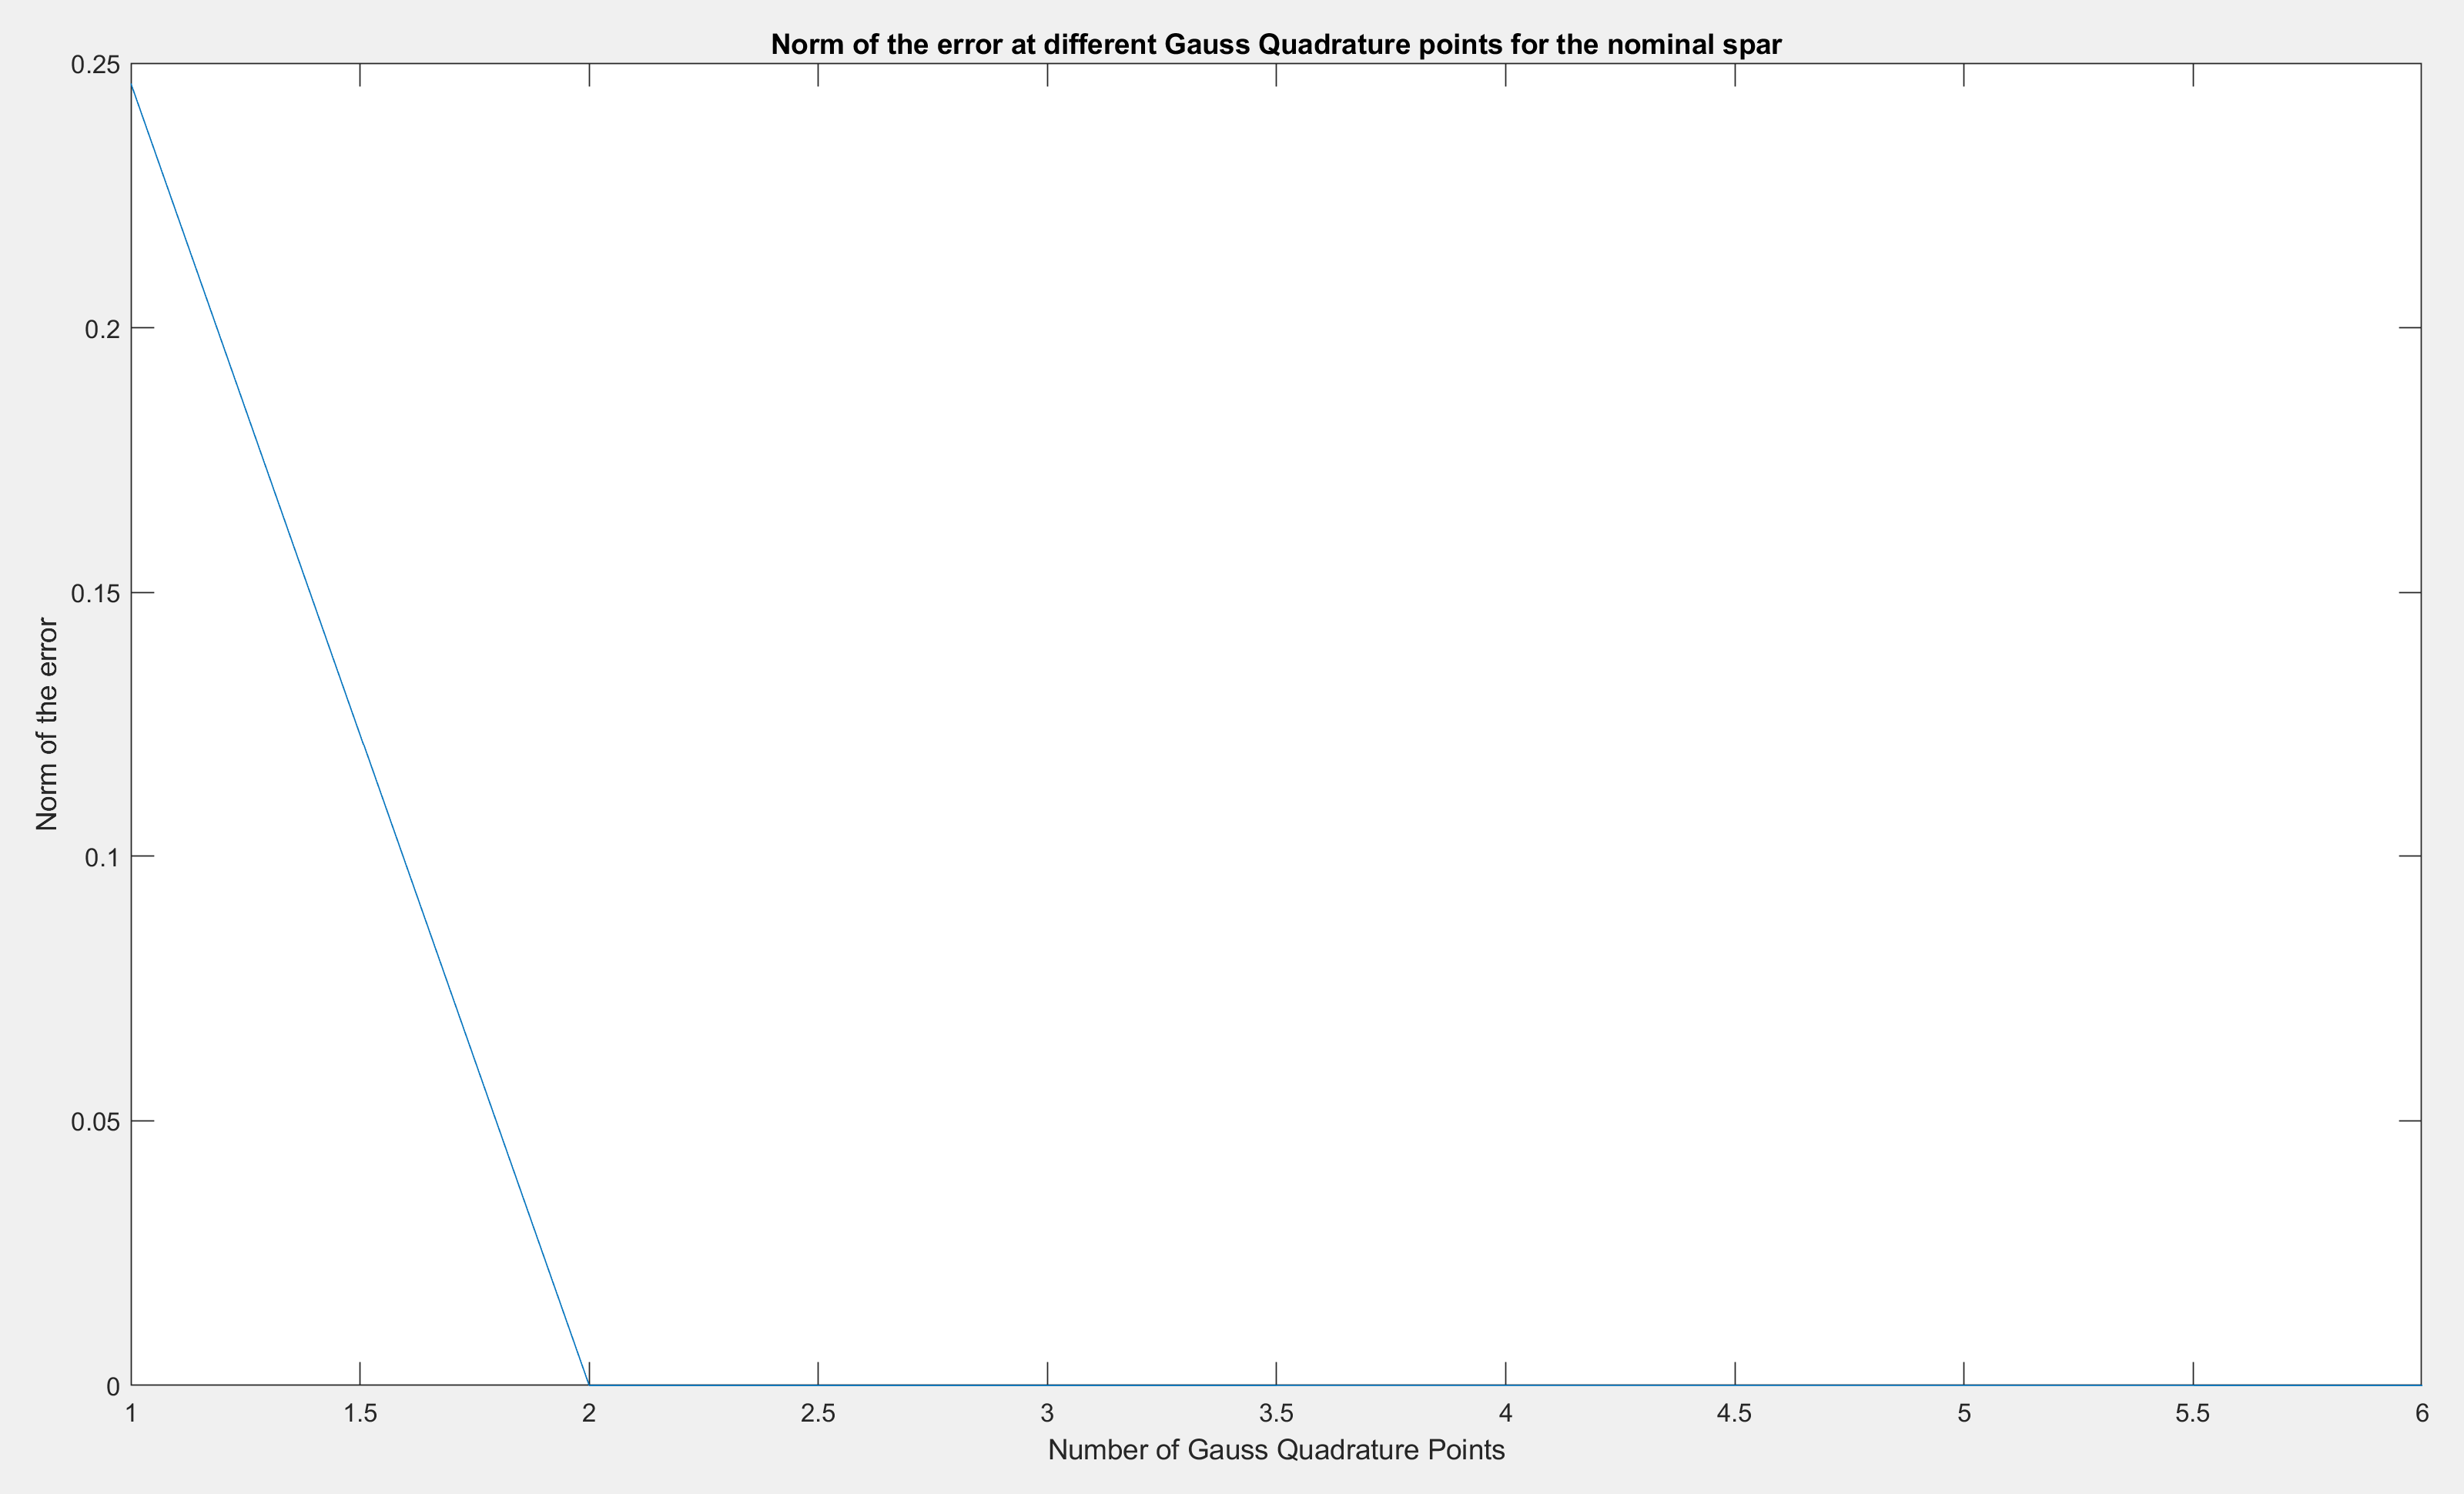
\includegraphics[width=0.75\linewidth]{conv.png}
    \caption{ Plot of the stress error vs Number of Gauss Quadrature points }
    \label{fig:conv}
\end{figure}

Once the convergence study was run, a graph of the mean and standard deviation for the nominal design was created to verify the analysis method. This was compared to a provided graph on Piazza, which was similar enough to conclude the analysis was implemented correctly.

\begin{figure}[h!]
    \centering
   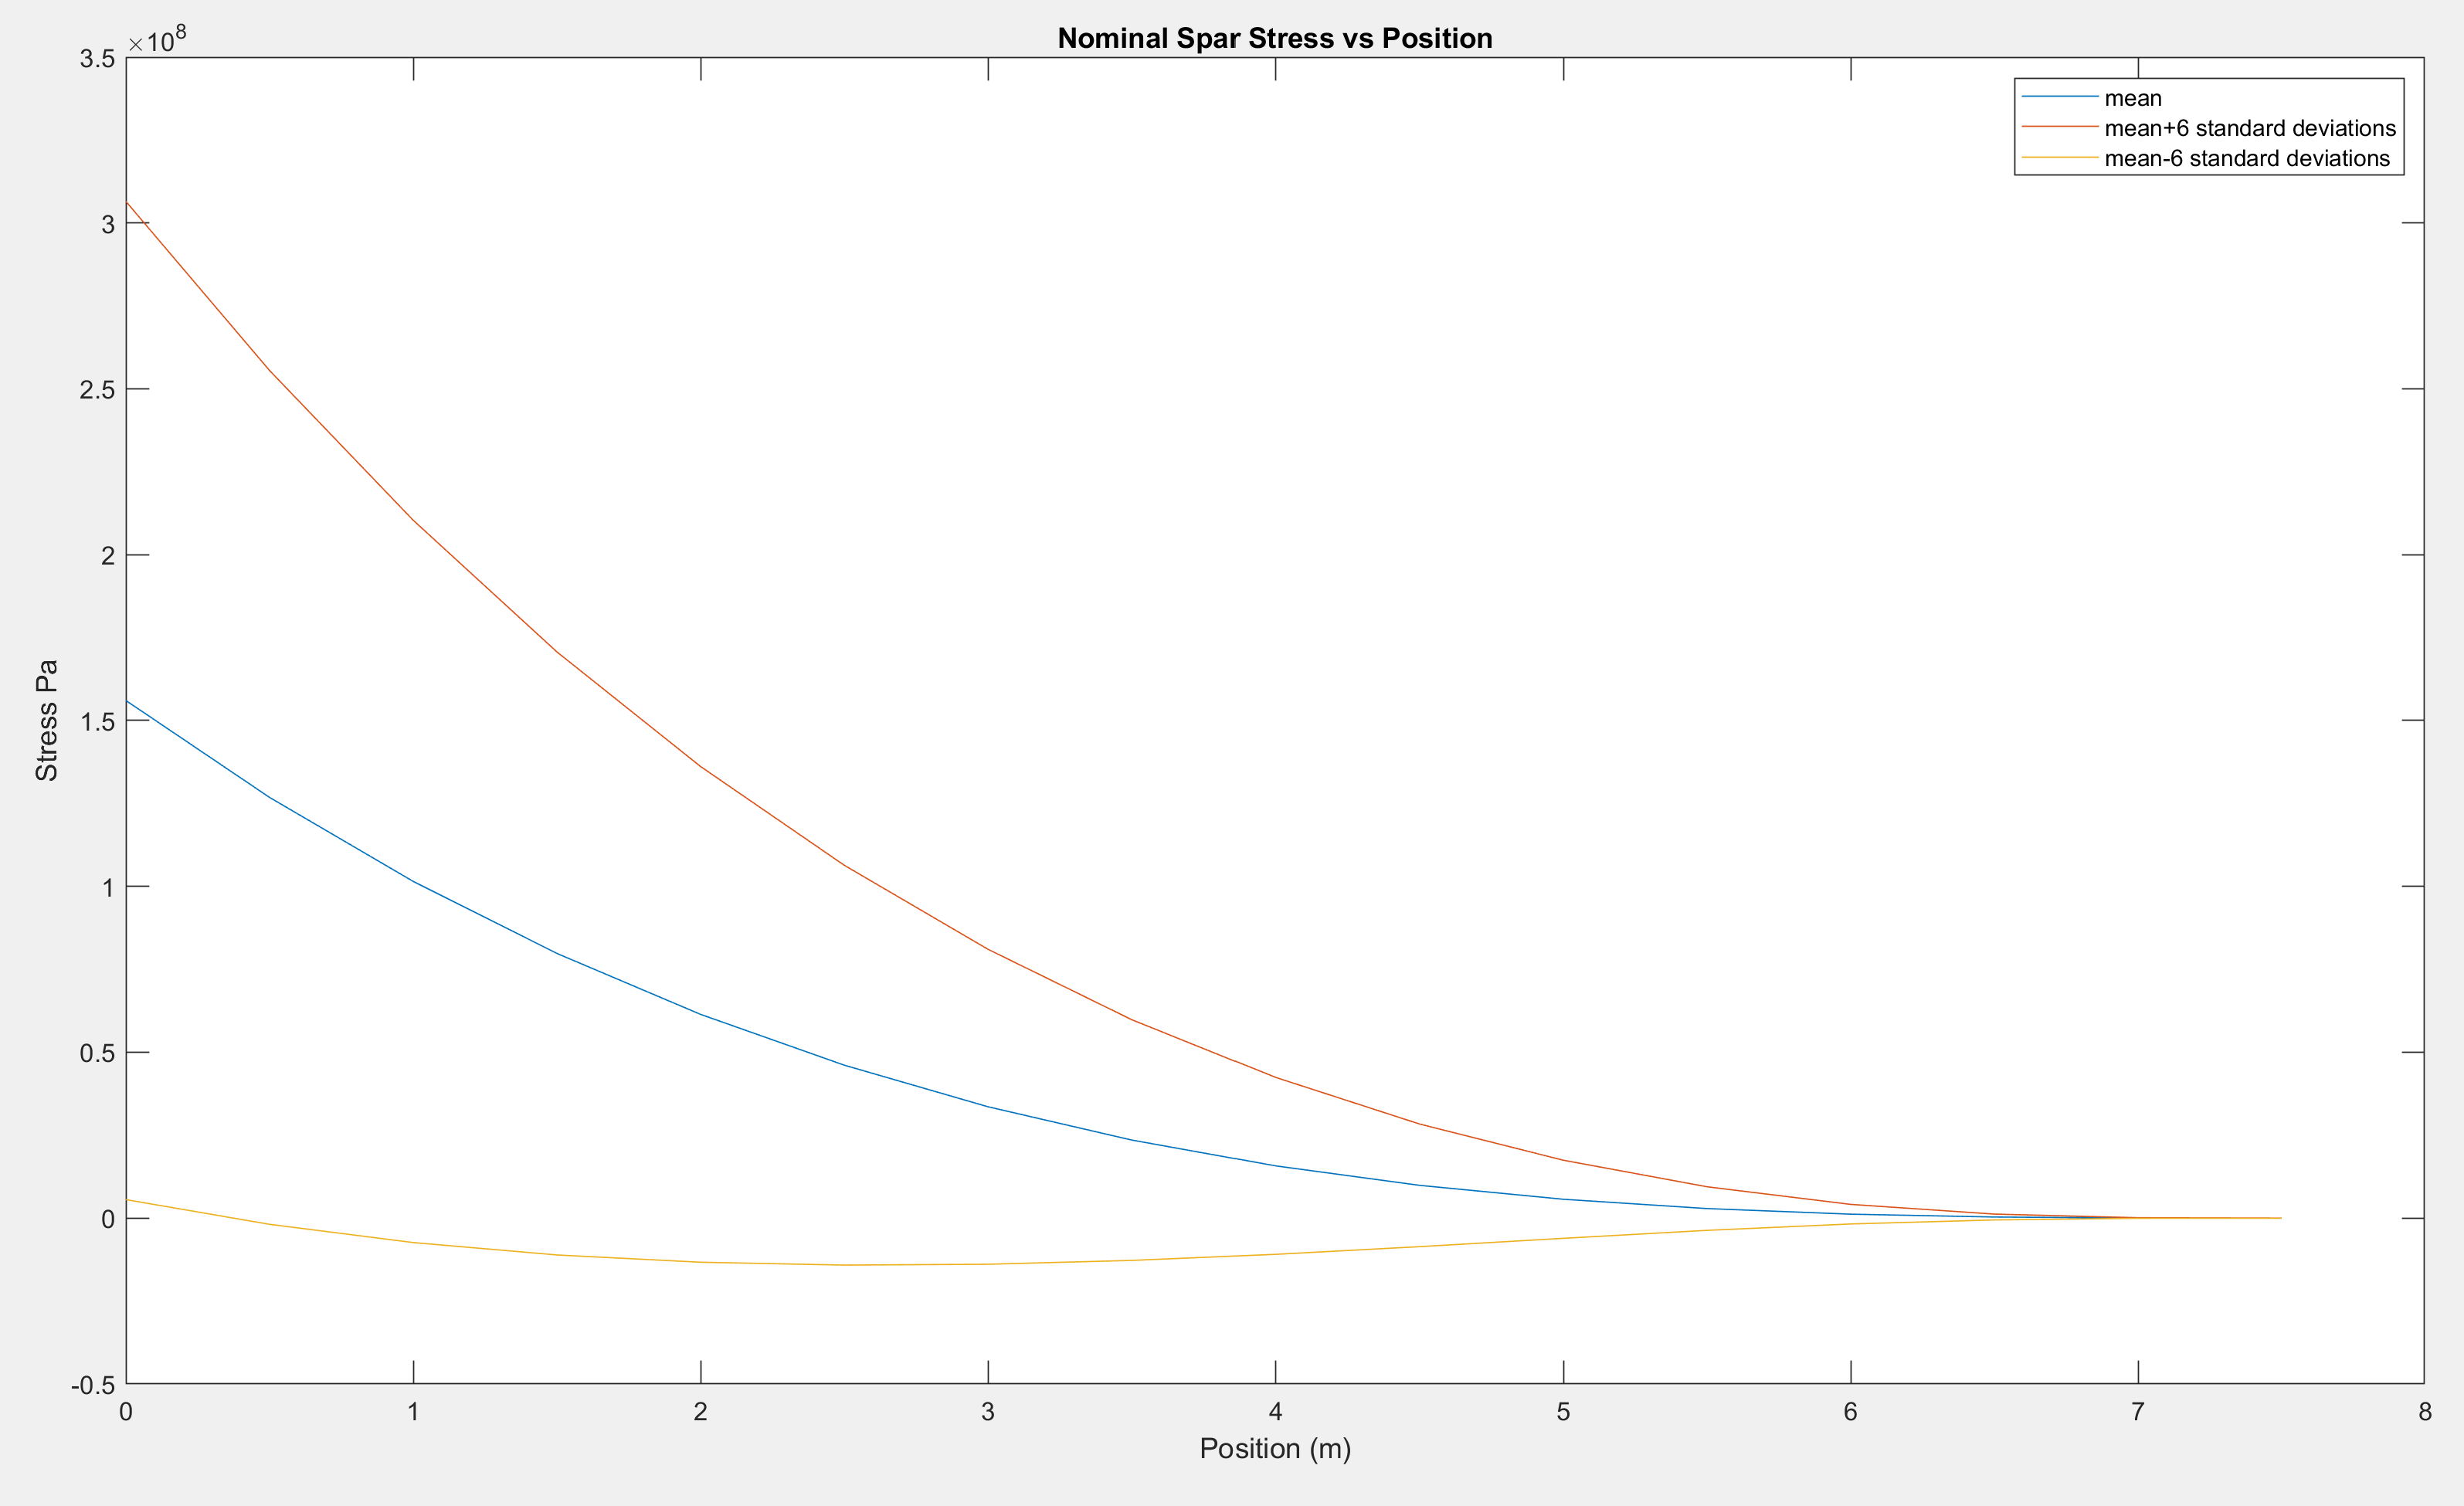
\includegraphics[width=0.75\linewidth]{nomstress.png}
    \caption{Stress vs Position in the Nominal Spar }
    \label{fig:nomstress}
\end{figure}
\newpage

The optimized shape of the wing spar with the chosen parameterization, number of elements (80)\cite{lab2}, and number of Gauss quadrature points (2) is shown in Figure \ref{fig:cross}. This result makes sense because it shows a similar inner and outer radii to the provided nominal design which gets thinner before the outer radii decrease until the design hits the lower bound of the design space, which would result in a limited mass of the spar. This is similar to the result from lab two shown in Figure \ref{fig:crossold}, except starting with a thicker initial portion at the root. This causes the rest of the design to be shifted towards the spar tip, which makes sense. This is because by adding uncertainty to the spar loading and designing for six standard deviations above the mean instead of designing for the mean, the effective applied force is increased resulting in a thicker spar with the same behavior.

\begin{figure}[h!]
    \centering
    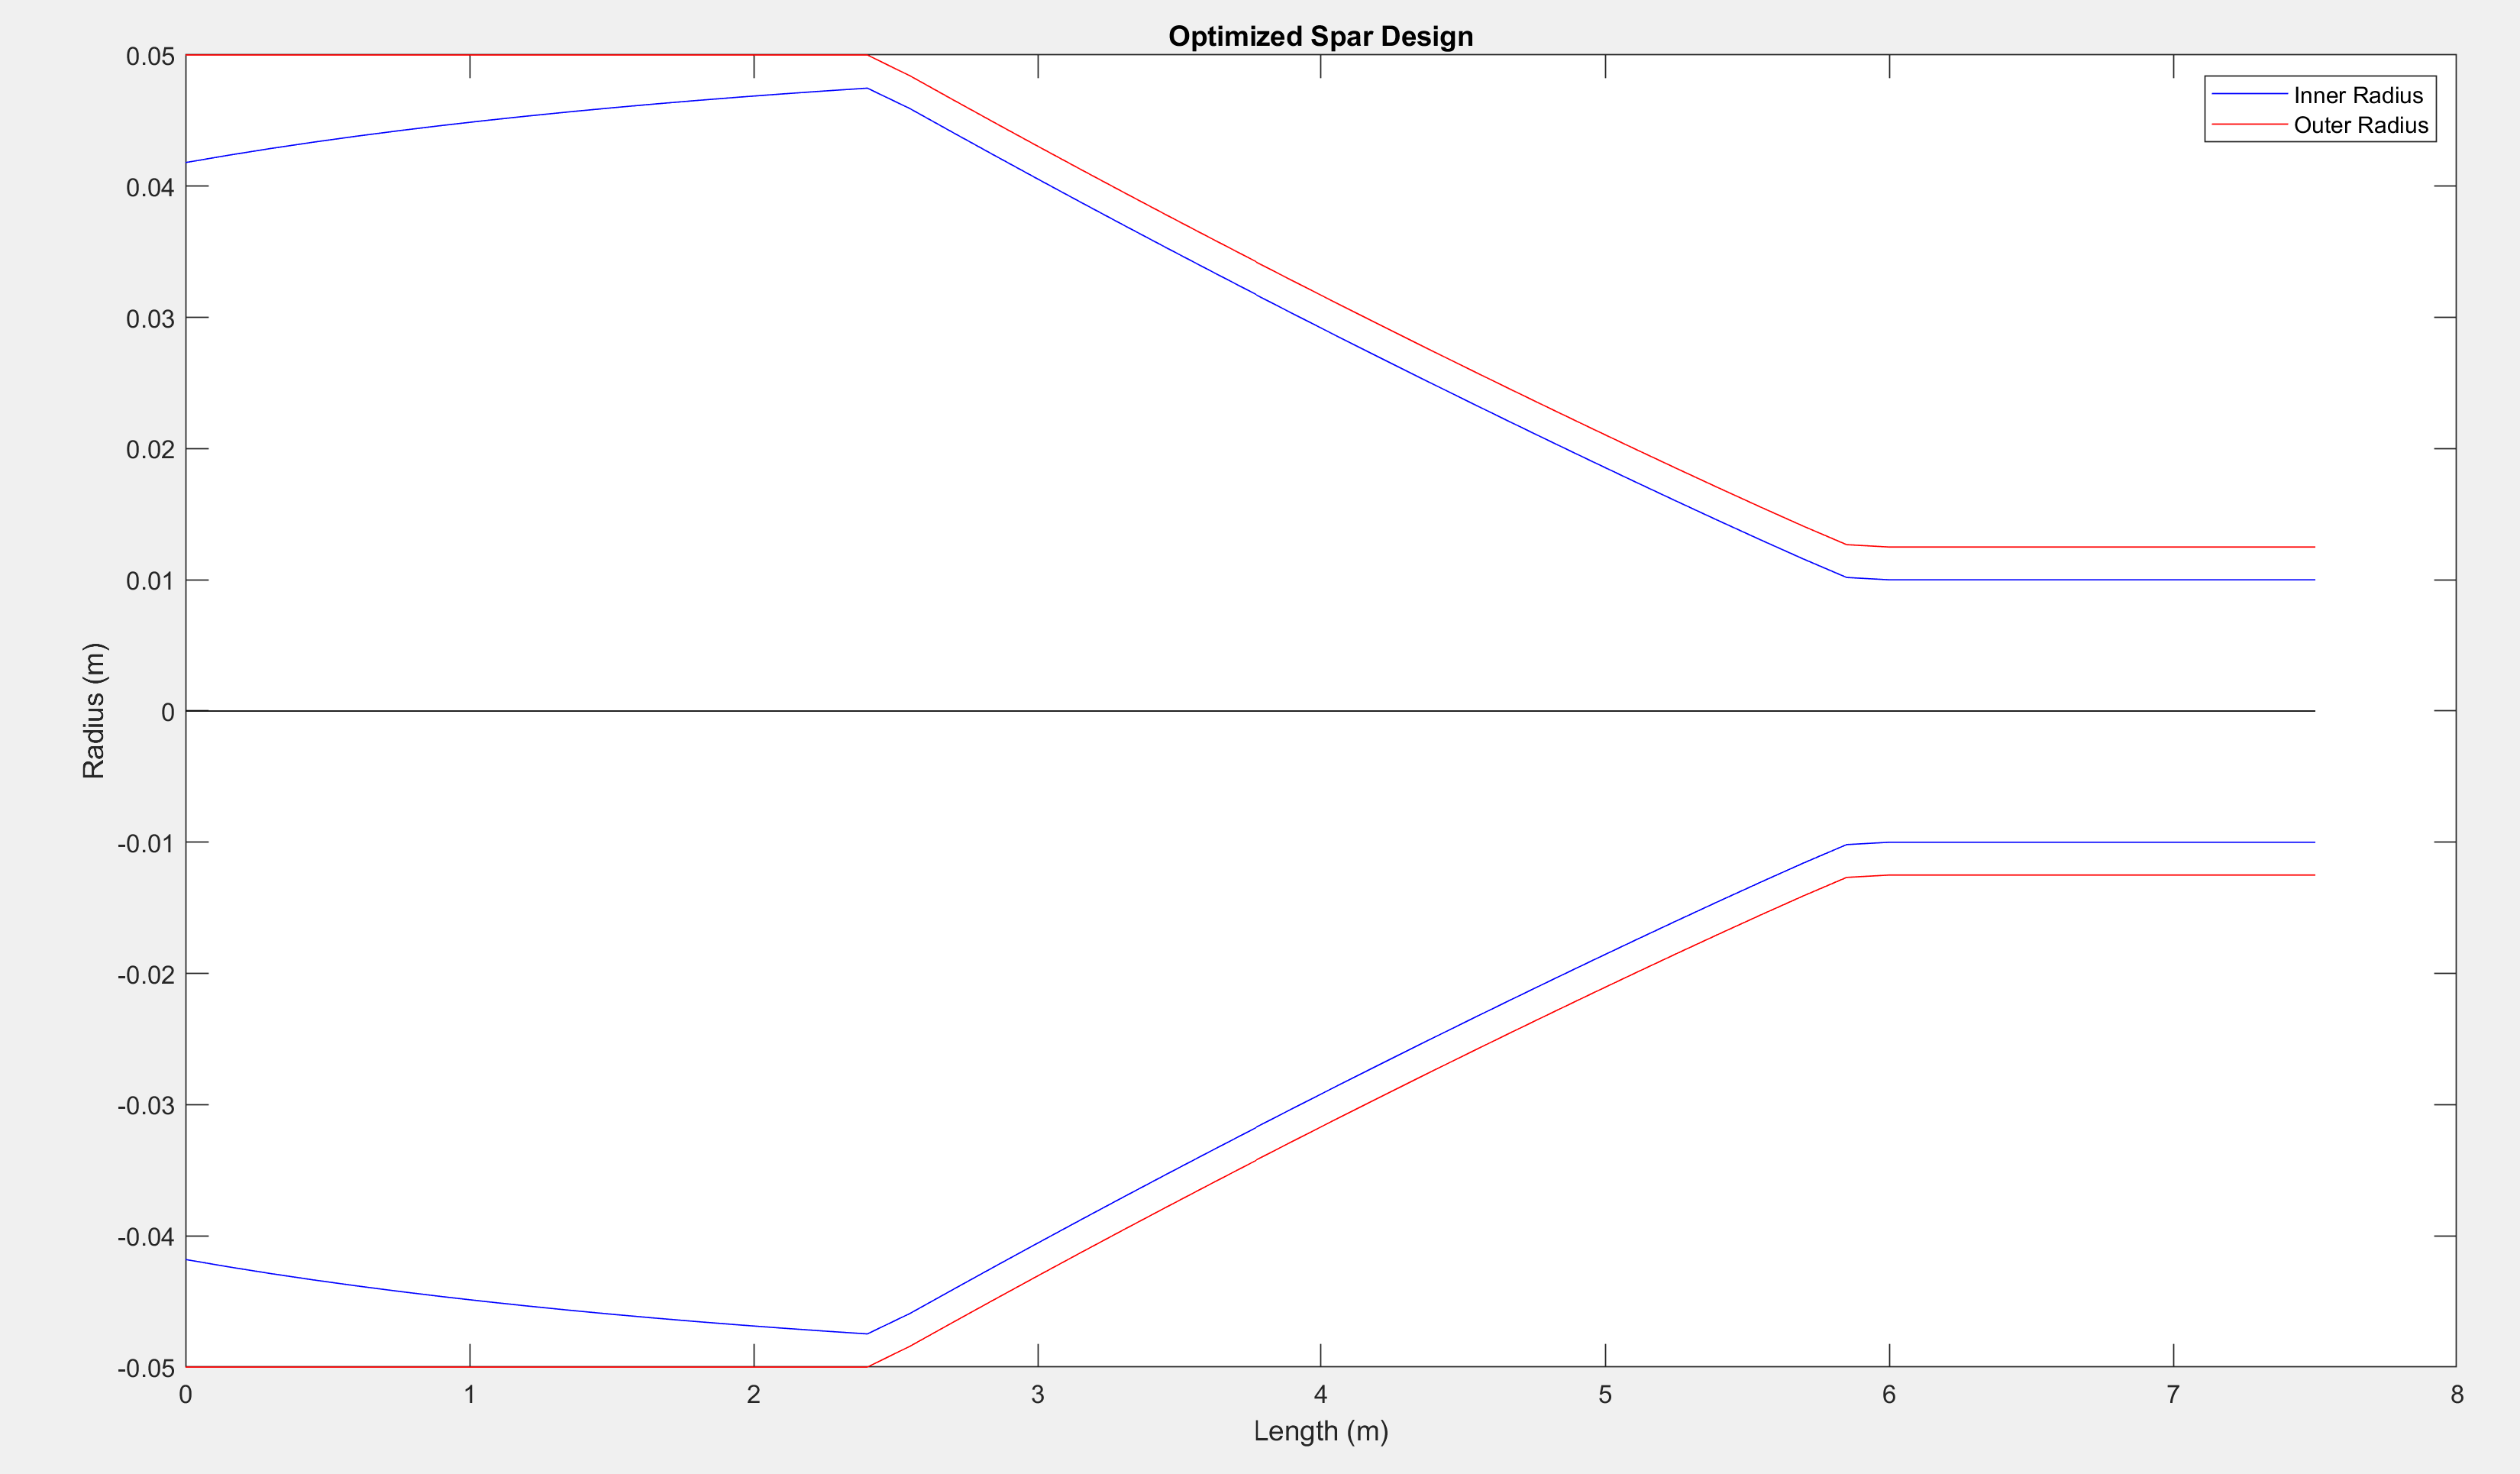
\includegraphics[width=0.75\linewidth]{fminconoutput.png}
    \caption{ Plot of the Wing Spar Cross Section }
    \label{fig:cross}
\end{figure}

\begin{figure}[h!]
    \centering
    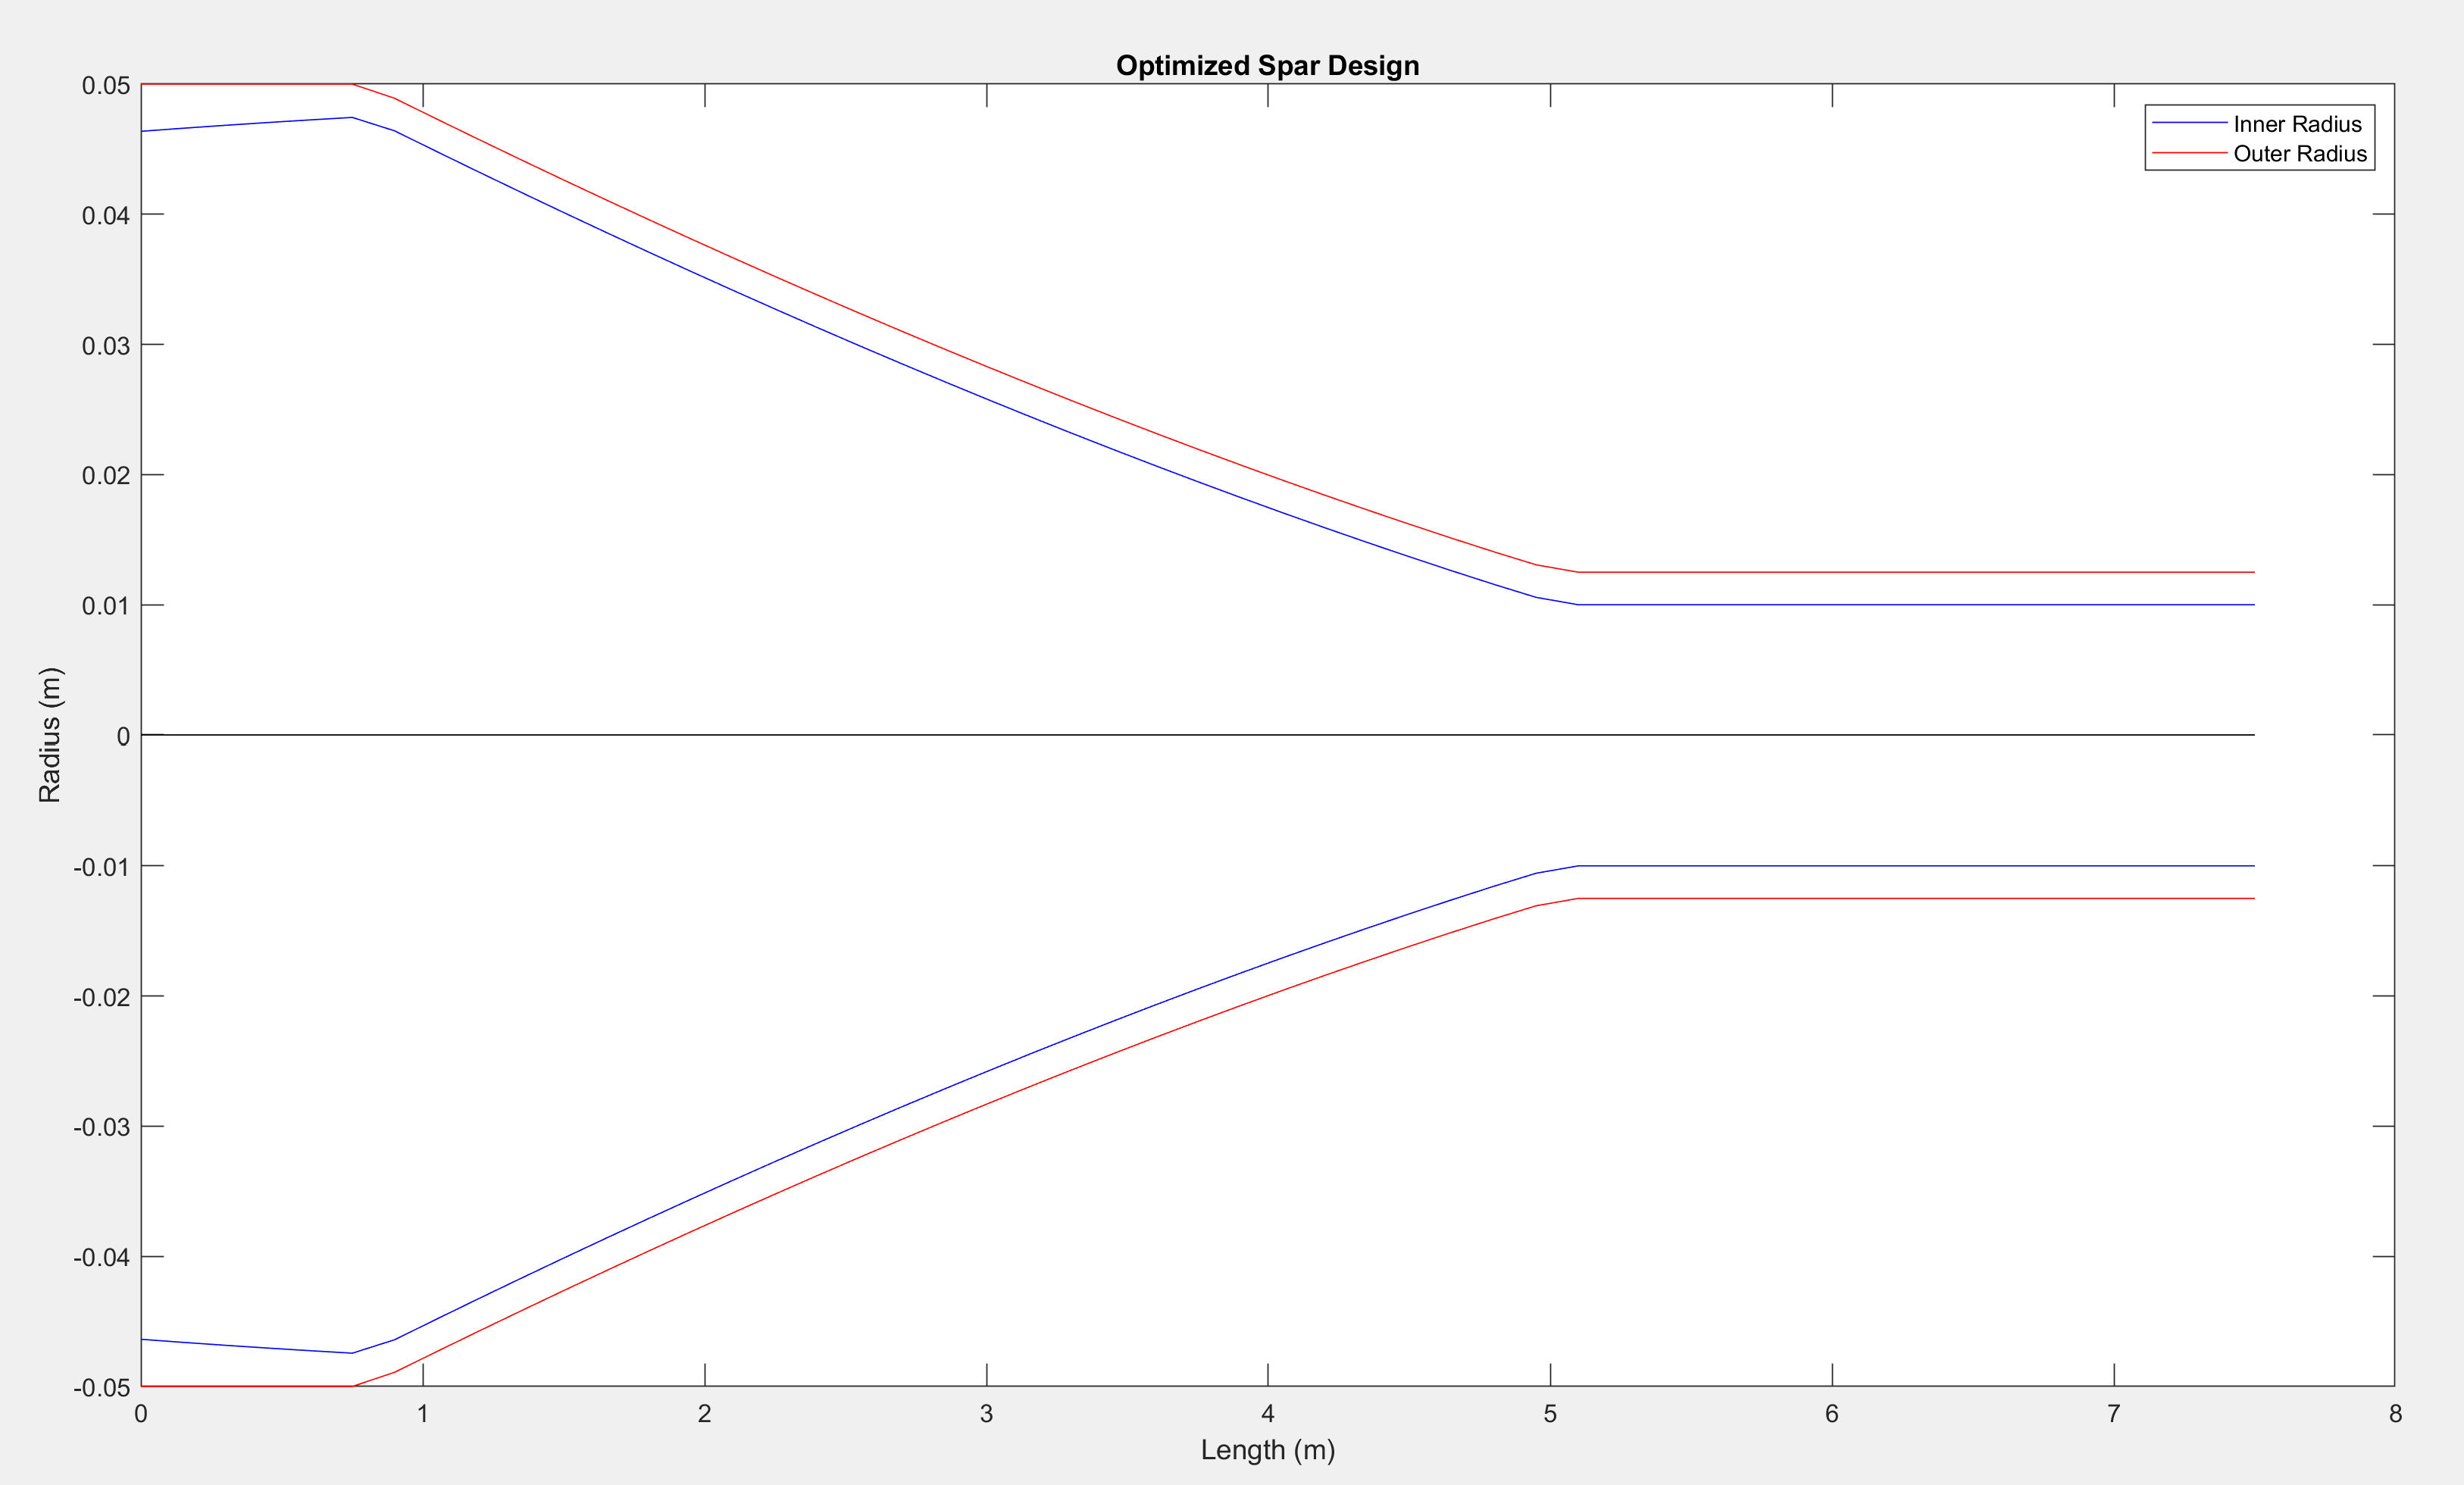
\includegraphics[width=0.75\linewidth]{fmiconoutput.png}
    \caption{ Plot of lab two's Wing Spar Cross Section }
    \label{fig:crossold}
\end{figure}

\newpage

The convergence plot shows that the First-Order Optimality score of the current solution decreased gradually over the first 12 iterations before rapidly decreasing as the optimization algorithm closed in on the solution (see Figure \ref{fig:feas}  the First Order Optimality decreased by six orders of magnitude over the iterations). (Note: the feasibility score for the optimization is 0 at every point, so the semilog plot didn't work for it). Also included is a of the mean and standard deviations of the stress at each node for the optimal design (figure \ref{fig:optstress}) (Note: the mean+6 standard deviations line behaves like the stress curve from lab 2 \cite{lab2}).

\begin{figure}[!ht]
    \centering
   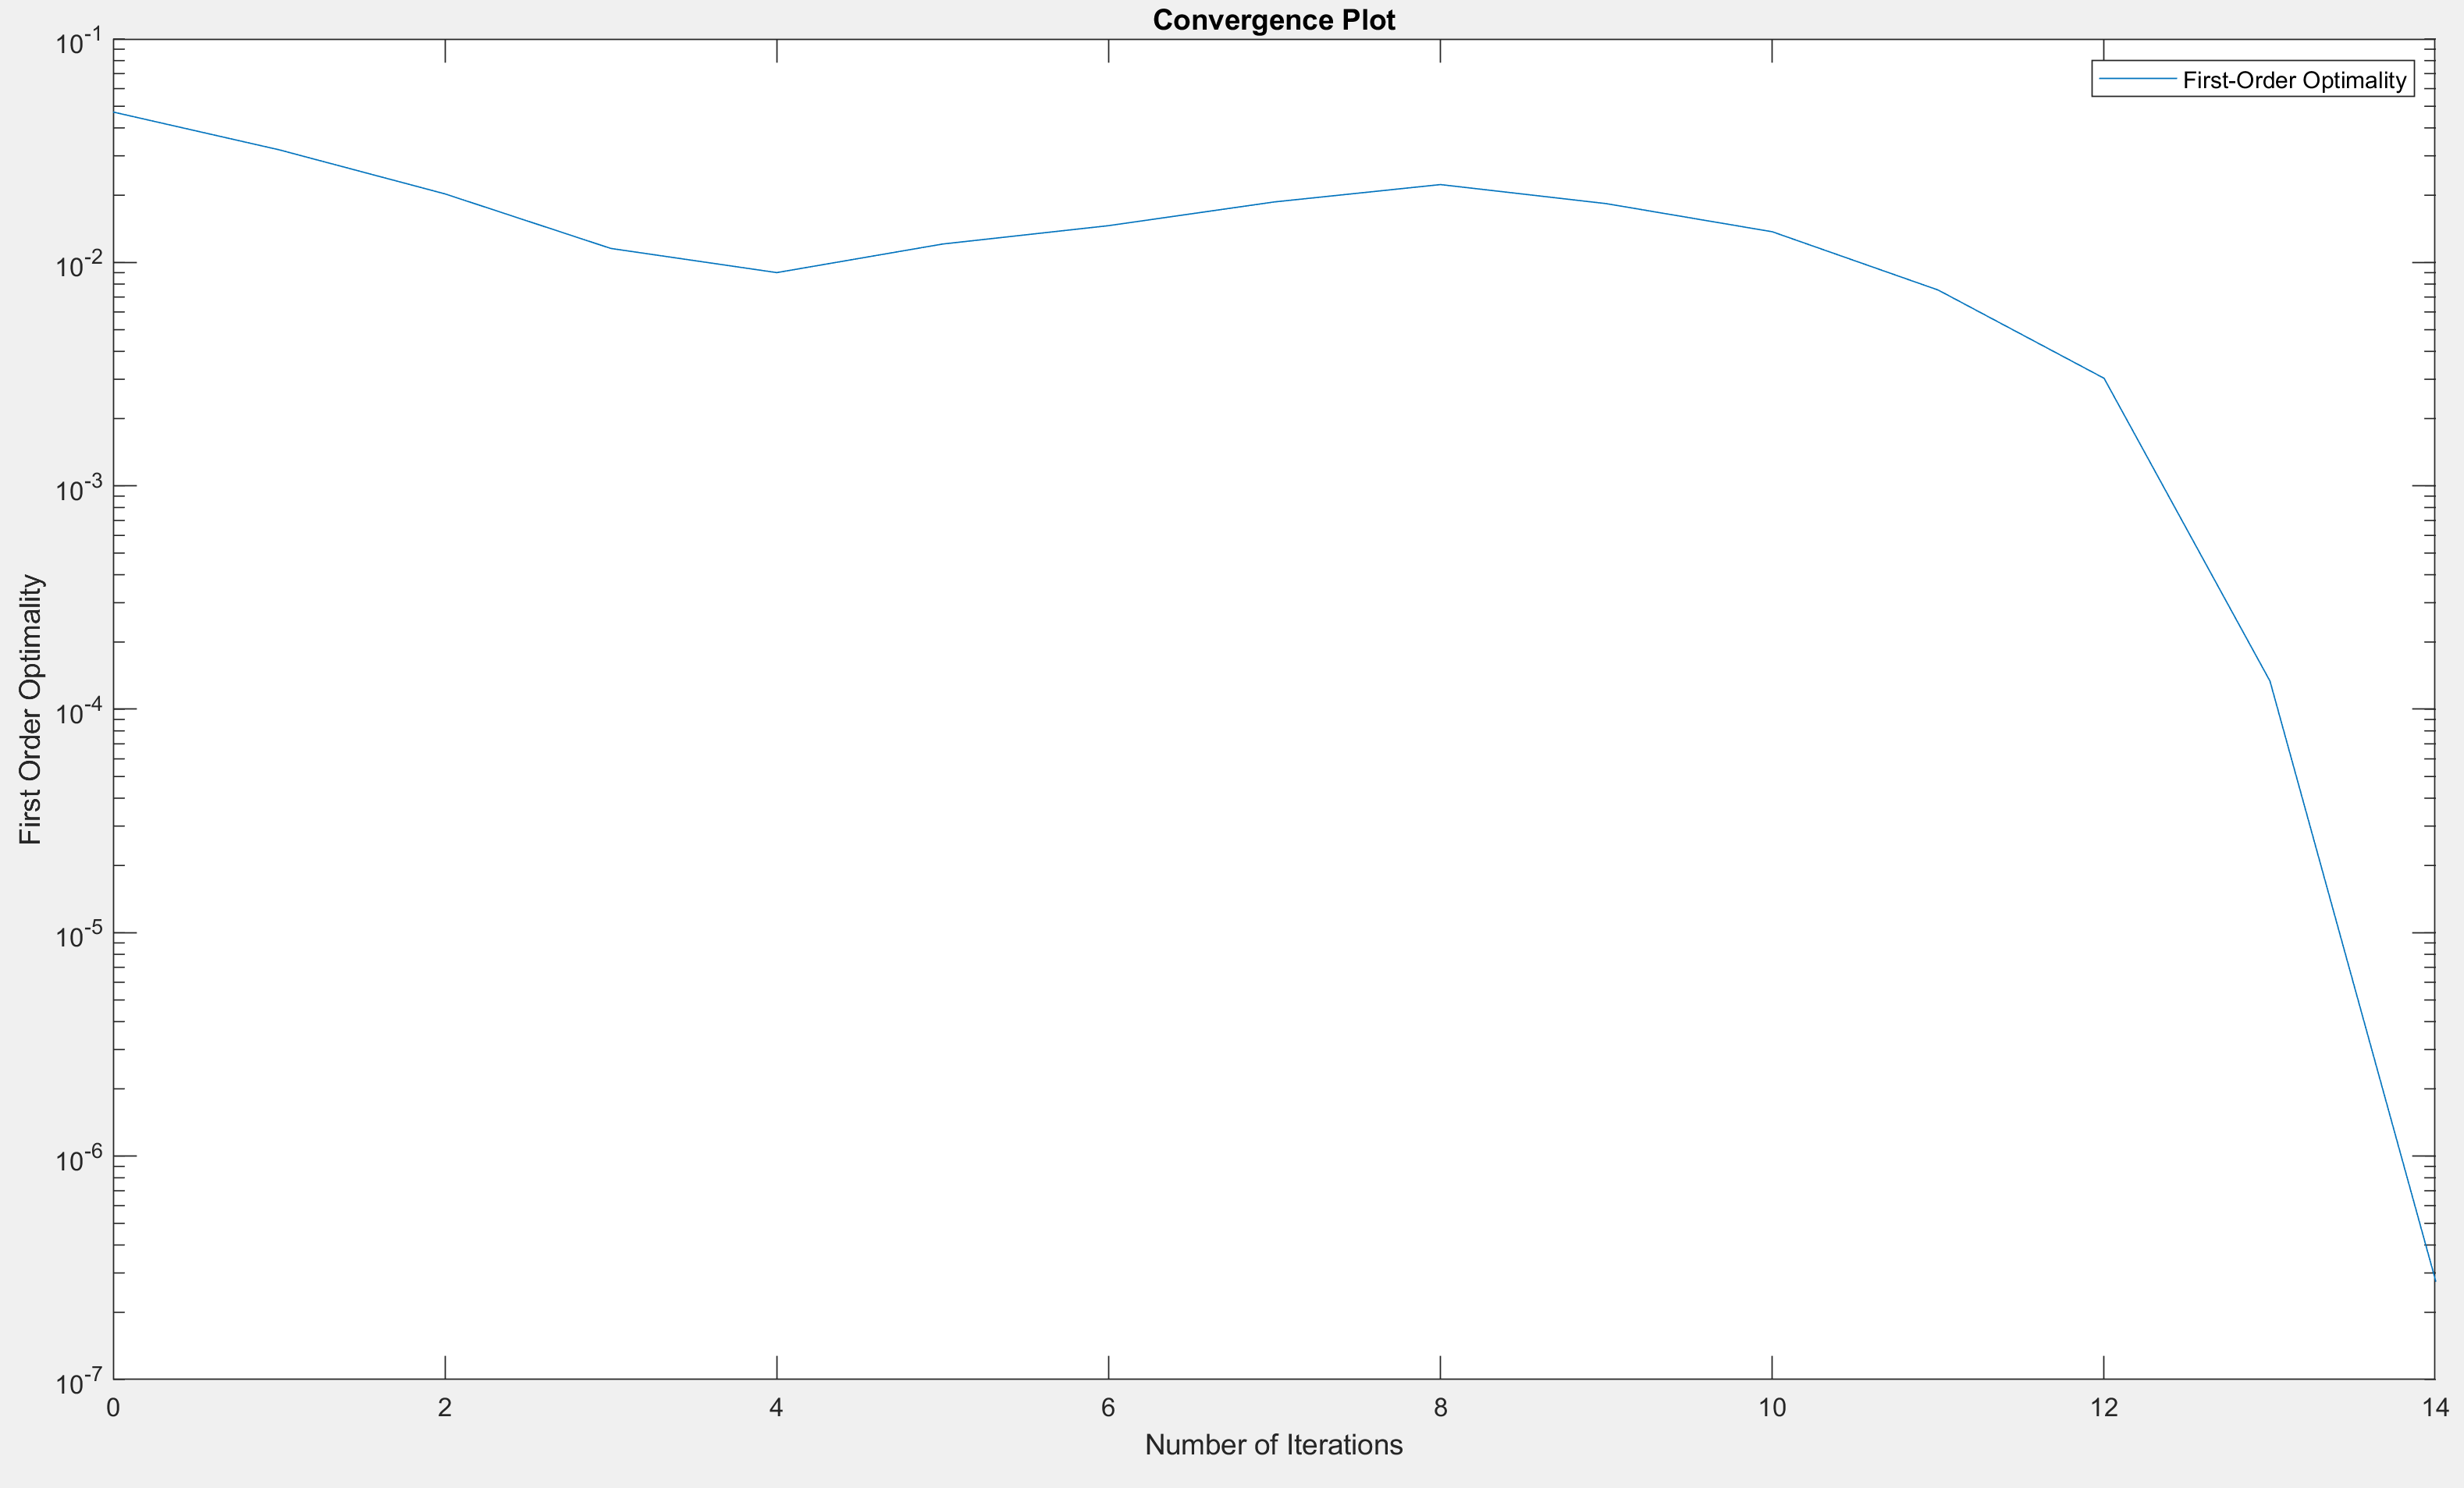
\includegraphics[width=0.75\linewidth]{firstorderopt.png}
    \caption{First order Optimality Convergence Plot }
    \label{fig:feas}
\end{figure}
\newpage
%mu+-6sd optimal
\begin{figure}[h!]
    \centering
   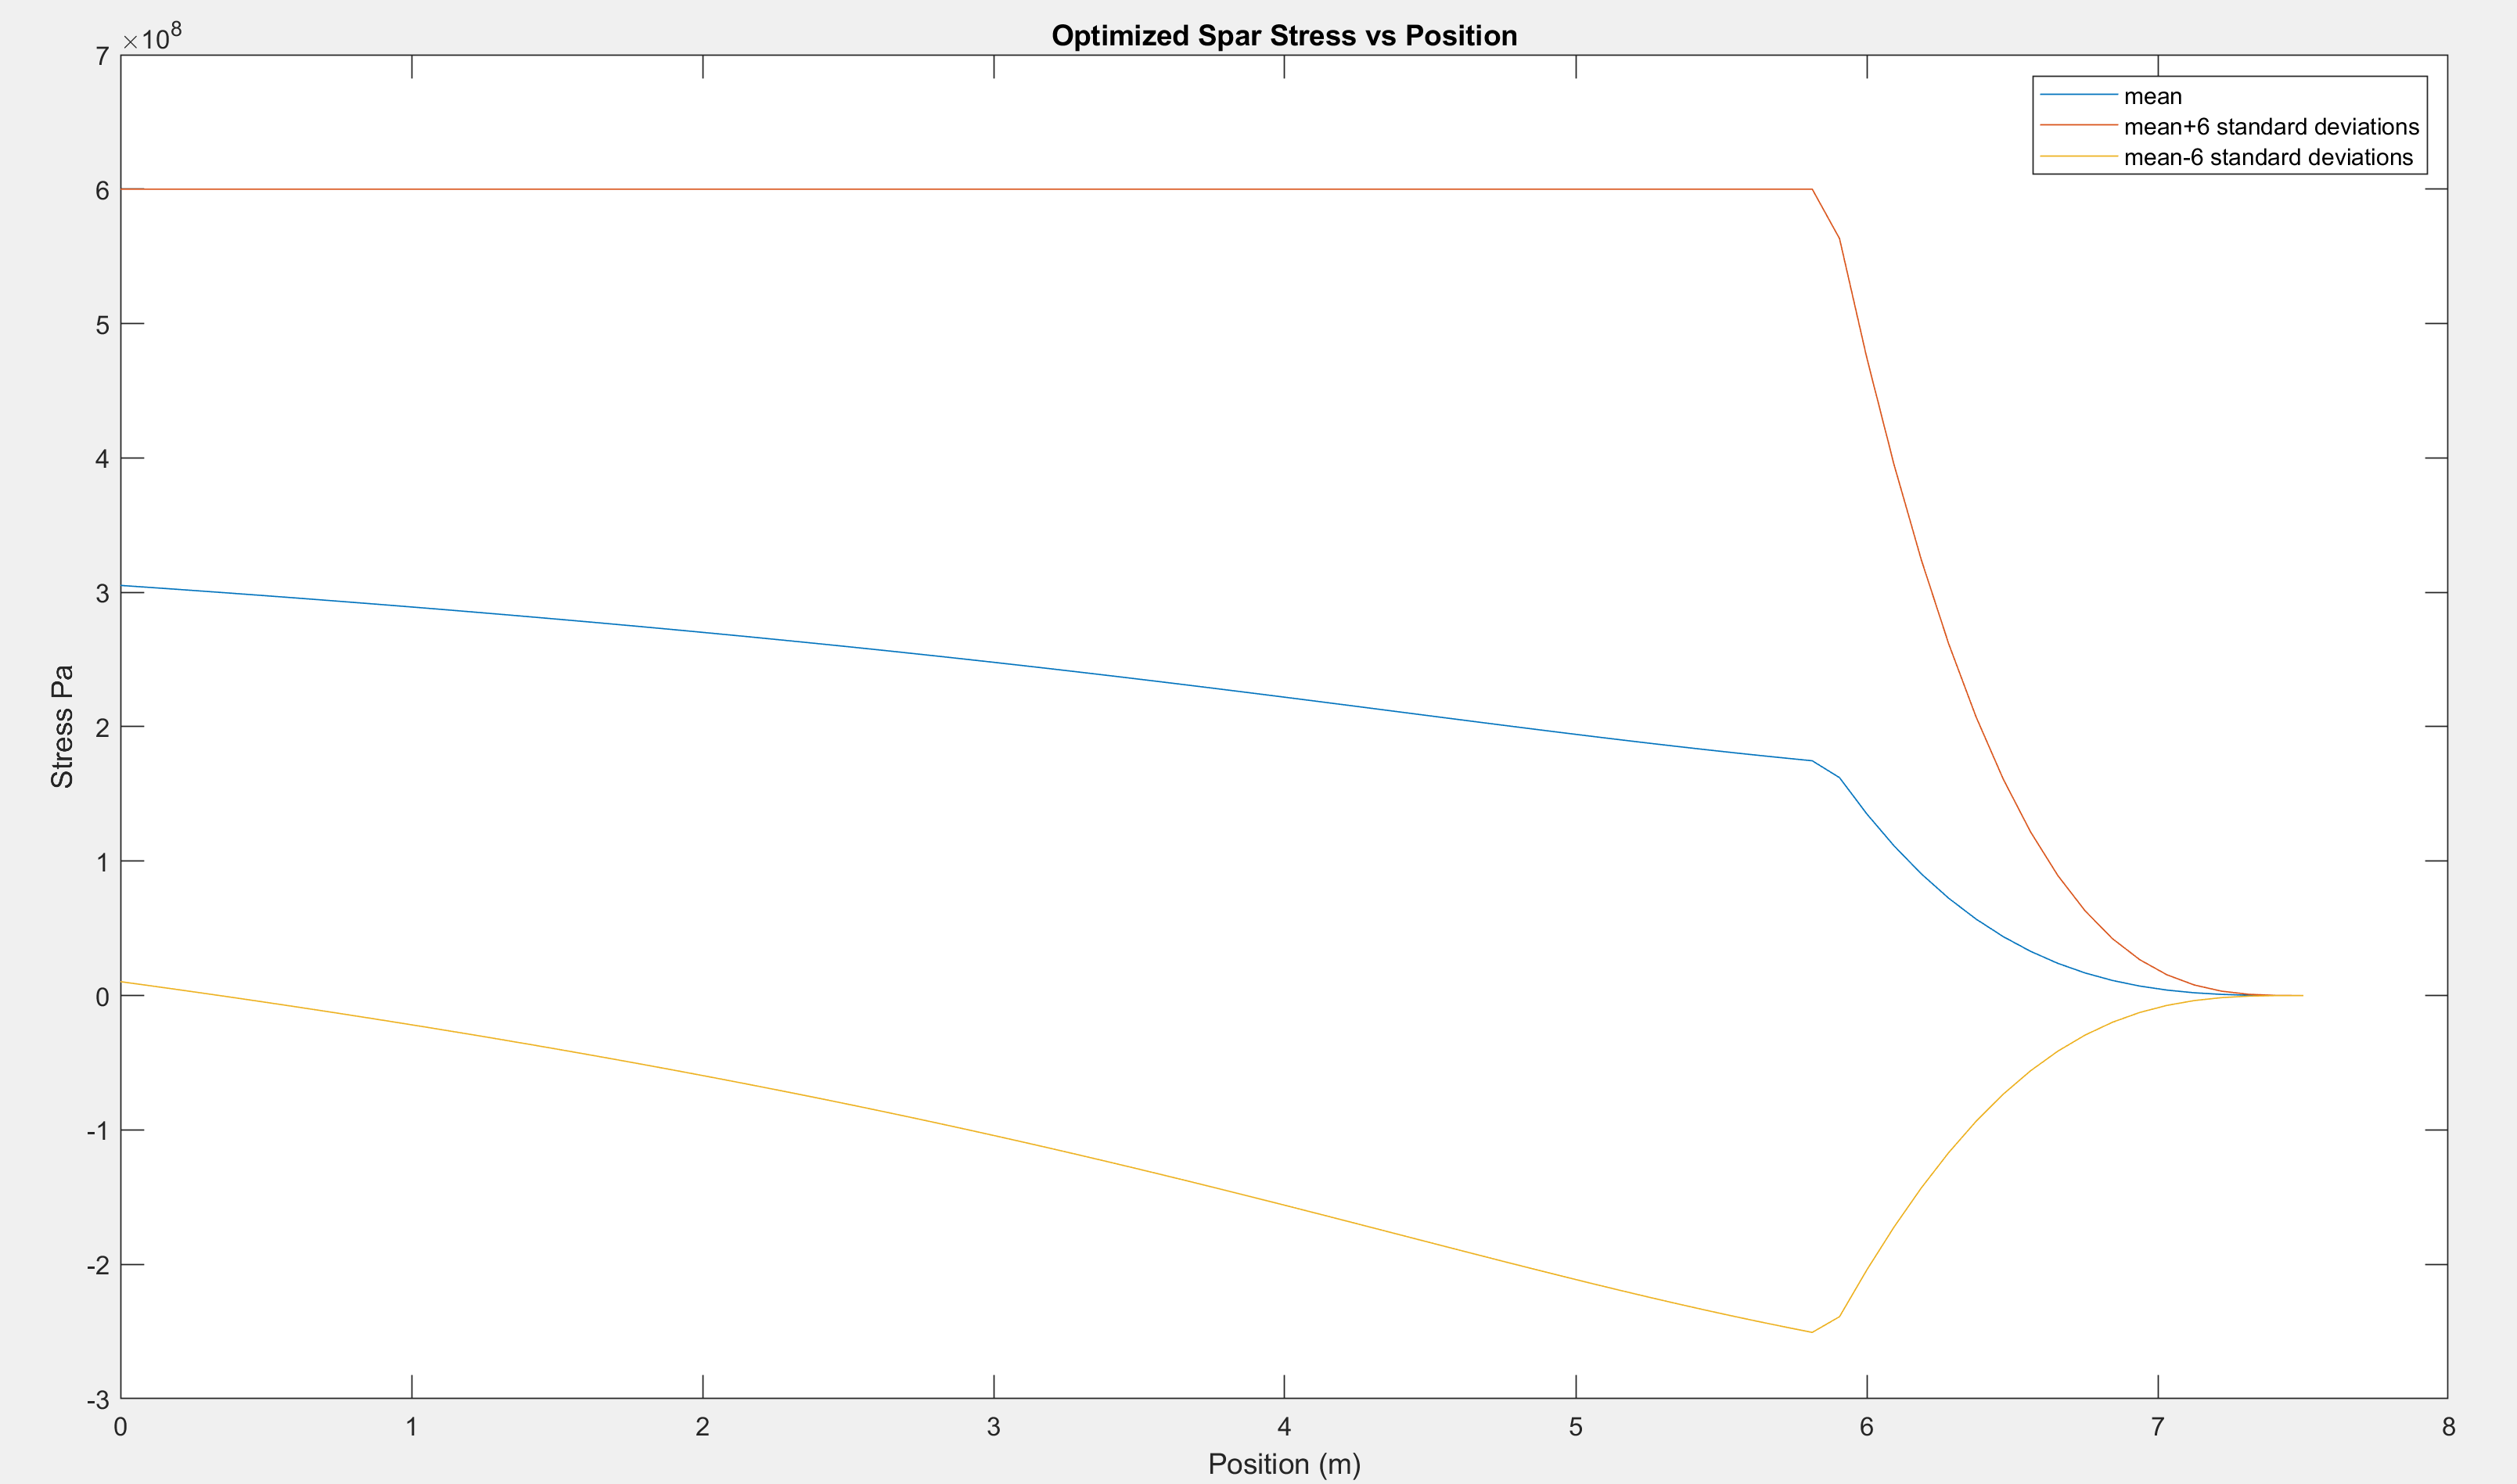
\includegraphics[width=0.75\linewidth]{optstress.png}
    \caption{Stress vs Position in the Optimized Spar }
    \label{fig:optstress}
\end{figure}
%mu+-6sd nominal

\medskip


\section{Conclusions}
The implementation of the SQP optimization algorithm with the complex step gradient method for this lab was successful. The resulting shape function for the optimized wing spar section profile made sense because it minimized the mass by minimizing the thickness and outer radius of the spar. The resulting calculated mass from the optimized wing spar was less than thirty percent of the baseline design ($0.3*29.32=8.796 > 8.784 $ kg) while remaining within the problem constraints. 

 Basic optimization algorithms, such as the ones used in this lab, can be powerful tools for understanding the complex interactions between different design variables in engineering design problems and balancing the design variables to arrive at an optimal solution. However, many engineering problems display uncertainty caused by noise in measured data. This lab demonstrated effective methods for handling these uncertainties while using optimization algorithms to prevent the creation of designs that only work in theory due to their lack of robustness. 

\addcontentsline{toc}{section}{References}
\printbibliography
\newpage
\section{Appendix}

\lstset{language=Matlab,%
    %basicstyle=\color{red},
    breaklines=true,%
    morekeywords={matlab2tikz},
    keywordstyle=\color{blue},%
    morekeywords=[2]{1}, keywordstyle=[2]{\color{black}},
    identifierstyle=\color{black},%
    stringstyle=\color{mylilas},
    commentstyle=\color{mygreen},%
    showstringspaces=false,%without this there will be a symbol in the places where there is a space
    numbers=left,%
    numberstyle={\tiny \color{black}},% size of the numbers
    numbersep=9pt, % this defines how far the numbers are from the text
    emph=[1]{for,end,break},emphstyle=[1]\color{red}, %some words to emphasise
    %emph=[2]{word1,word2}, emphstyle=[2]{style},    
}
\subsection{getq.m}
\label{sec:getq}
\lstinputlisting{code/getq.m}
\newpage
\subsection{run.m}
\label{sec:run}
\lstinputlisting{code/run.m}
\newpage
\subsection{getR.m}
\label{sec:getR}
\lstinputlisting{code/getR.m}
\newpage
\subsection{getI.m}
\label{sec:getI}
\lstinputlisting{code/getI.m}
\newpage
\subsection{getC.m}
\label{sec:getC}
\lstinputlisting{code/getC.m}
\newpage
\subsection{putR.m}
\label{sec:putR}
\lstinputlisting{code/putR.m}
\newpage
\subsection{calcVol.m}
\label{sec:calcVol}
\lstinputlisting{code/calcVol.m}
\newpage
\subsection{plots.m}
\label{sec:plots}
\lstinputlisting{code/plots.m}
\subsection{fmincon Output}
\label{sec:fincon}
\begin{figure}[h!]
    \centering
    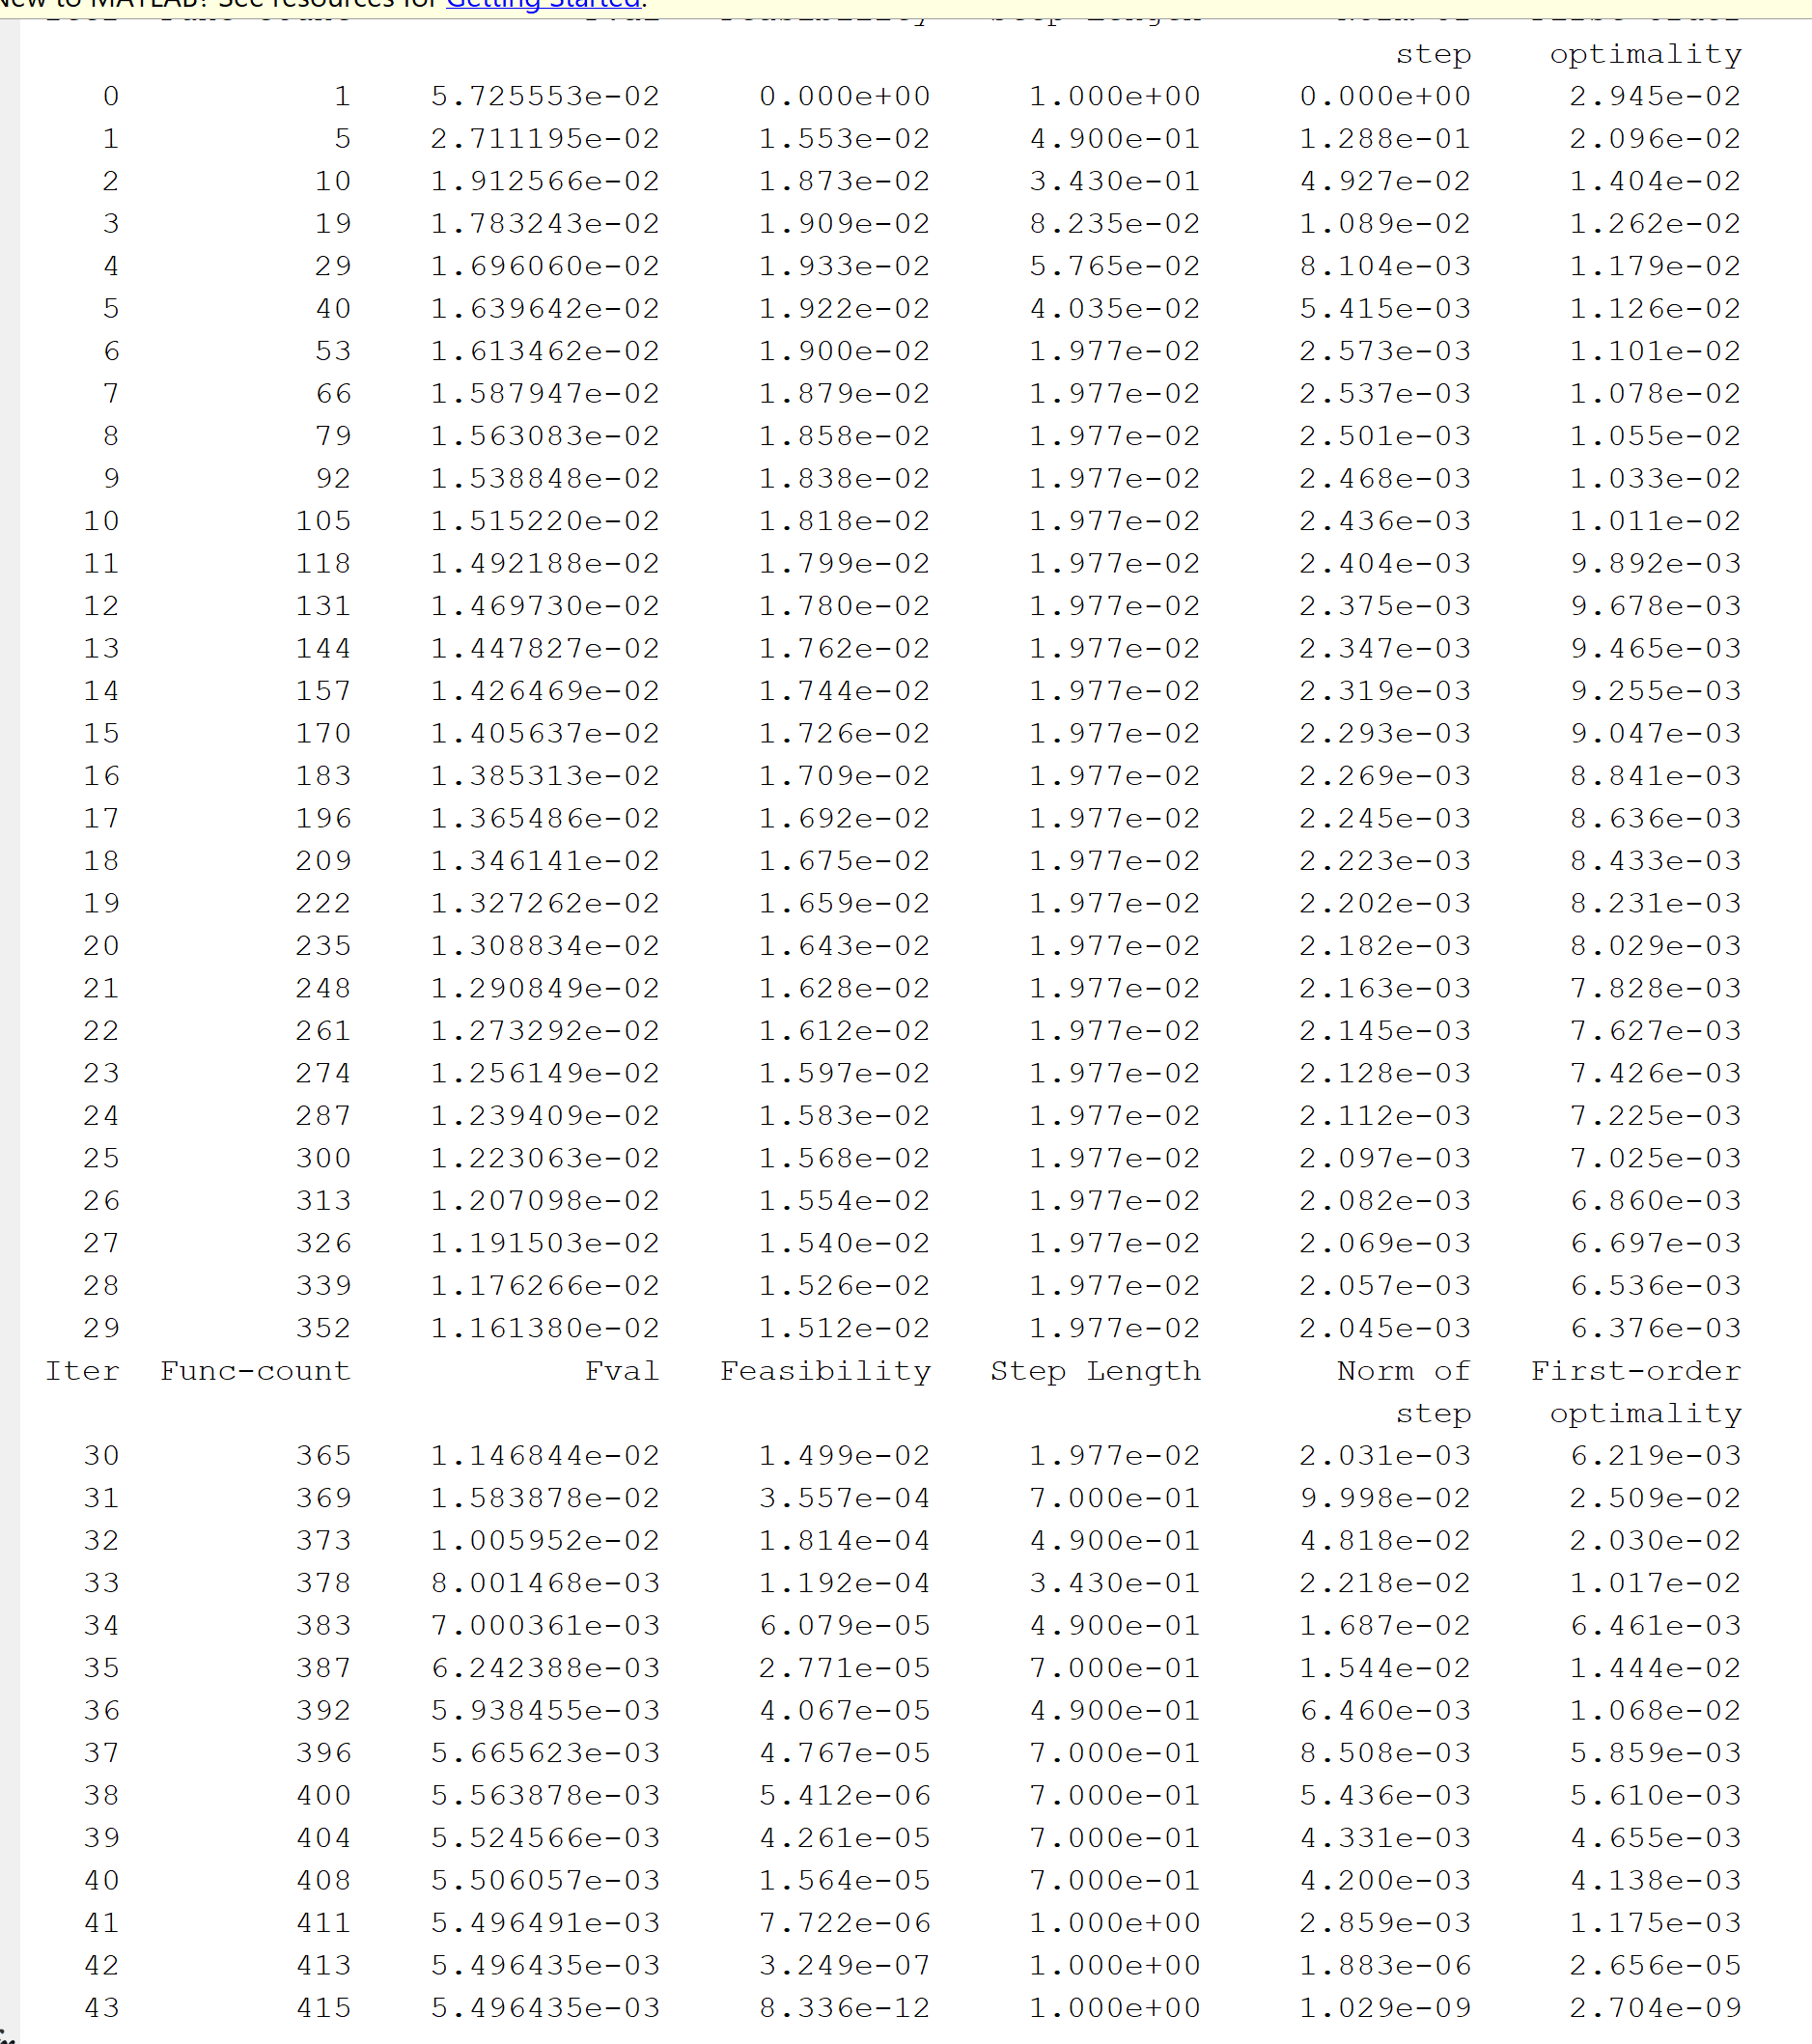
\includegraphics[width=0.75\linewidth]{out.png}
    \caption{ The Outpt of fmincon }
    \label{fig:fmincon}
\end{figure}

\end{document}